\section{Results}
\label{sec:results}

The results are given in the order of the hypotheses. Every number in this section is written by a committed script from the outputs of the experiments, and the main comparison is Table~\ref{tab:main-results}.

\begin{table}[htbp]
\centering
\small
\caption{Main comparison: each component of the engine against the independent reference run on the same input, with the repetition uncertainty (plus or minus one standard deviation) where the quantity is random; z is the difference of the two means over its standard error.}
\label{tab:main-results}
\begin{tabular}{p{2.8cm}p{3.2cm}p{2.7cm}p{2.9cm}p{2.3cm}}
\toprule
Component & Quantity & Engine & Reference & Outcome \\
\midrule
\relax ECB statistics & \relax five statistics, independent transcription & \relax 5 of 17 sections & \relax largest difference $4.4\times 10^{-11}$ & \relax held (quadrature accuracy) \\
\relax ECB Jeffreys test, C01 holdout & \relax grades flagged at 5\%, all models & \relax 4 of 70 & \relax binomial 3 of 70 & \relax 1 cell differs \\
\relax Large-portfolio law & \relax density integral against distribution function & $4.3\times 10^{-12}$ & \relax adaptive quadrature & \relax held \\
\relax IRB capital & \relax credit-card book, retail revolving & \relax 0.039170 & \relax SciPy formula, difference 0 & \relax held \\
\relax CreditRisk+ recursion & \relax mean, variance, probability of no loss & \relax variance gap $5.5\times 10^{-11}$ & \relax independent recursion $3.1\times 10^{-17}$ & \relax held \\
\relax Granularity adjustment & \relax delta at xi 0.25, level 0.999 & \relax 4.8336 & \relax published 4.83 & \relax held \\
\relax Gaussian copula, 99.9\% VaR & \relax 10 runs of 200,000 & \relax 3,193,200 $\pm$ 23,925 & \relax independent 3,187,800 $\pm$ 31,119 & \relax z +0.44 \\
\relax Gaussian copula, 99\% ES & \relax 10 runs of 200,000 & \relax 2,576,013 $\pm$ 15,358 & \relax independent 2,572,709 $\pm$ 18,338 & \relax z +0.44 \\
\relax Committed seeded rung & \relax 1,000,000 scenarios, eight values & \relax relative difference $2.9\times 10^{-9}$ & \relax committed file & \relax held \\
\relax Importance sampler & \relax 20 seeds, P(L at or above 99.9\% VaR) & \relax 0.00106 $\pm$ $6.9\times 10^{-6}$ & \relax plain 0.00104 $\pm$ 0.00008 & \relax z +1.06, variance ratio 146 \\
\relax Correlation estimator, 24 cells & \relax coverage of the 95\% interval, maximum likelihood & \relax mean 0.942, lowest 0.912 & \relax band $\pm$0.028 & \relax 1 of 24 cells outside; 16 below 0.95 \\
\relax Correlation estimator, 24 cells & \relax coverage, moments & \relax mean 0.817 & \relax same band & \relax 24 of 24 cells outside \\
\relax IRRBB shock shapes & \relax SRP31.92 example, flattener & \relax -1.64 bp & \relax printed $-1.6$ bp & \relax deviation 0.039 bp \\
\relax IRRBB present values & \relax 72 leg and shock pairs, six variants & \relax relative difference $2.4\times 10^{-14}$ & \relax QuantLib & \relax held \\
\bottomrule
\end{tabular}
\end{table}


\subsection{What the catalogue holds and which ECB statistics it implements}

The registry of release \inventoryVersion{} holds \testsTotal{} tests in \familiesTotal{} families, \pvalueTests{} decided by a $p$-value and \metricTests{} by a metric, and every one has a non-empty primary source (Table~\ref{tab:catalogue}). Six of them cite the ECB instructions: the five statistics of Section~\ref{sec:proposed-method} and the area under the ROC curve with the ECB standard error. Table~\ref{tab:ecb-coverage} sets the \ecbSections{} statistics that the instructions fix against the registry. The engine implements \ecbImpl{} as specified, namely the Jeffreys test, the area against its development value, the matrix weighted bandwidth, the migration z-tests and the concentration test; \ecbRelated{} is implemented in a related but different form, the paired $t$-test of the loss given default, which in the engine is two-sided and by segment and not the one-sided test over the twelve fixed segments of the instructions; and \ecbAbsent{} are not implemented: the qualitative validation tools of the probability of default, of the loss given default and of the credit conversion factor (four groups of sections), the generalised area statistic of the loss given default and of the credit conversion factor, the loss-in-default and expected-loss best-estimate tests, the credit conversion factor and exposure back-tests and the slotting statistics. The \ecbSections{} entries are the author's reading of Sections 2.5 to 2.10 of the instructions, with one entry for each statistic, one for each group of qualitative validation tools (Sections 2.5.2, 2.6.4, 2.9.2 and 2.9.5) and one for the slotting section (2.10); the count of absent statistics depends on that grouping, and counting each qualitative sub-section as a statistic would raise it. The second part of Hypothesis~H1, that all statistics the instructions fix are implemented, is refuted: \ecbAbsent{} of \ecbSections{} are absent. The package implements the ECB statistics of the probability of default and not those of the loss and exposure parameters.

\begin{table}[htbp]
\centering
\small
\caption{Tests registered by the engine release 1.1.0, by family: 134 tests in 18 families, 42 decided by a p-value and 92 by a metric, each with its primary source.}
\label{tab:catalogue}
\begin{tabular}{lrlr}
\toprule
Family & Tests & Family & Tests \\
\midrule
aggregation & 8 & market & 12 \\
ccr & 8 & ml & 13 \\
discrimination & 4 & oprisk & 5 \\
fairness & 12 & pd-calibration & 11 \\
governance & 5 & portfolio & 5 \\
ifrs9 & 9 & rating-system & 3 \\
irrbb & 7 & stability & 5 \\
lgd-ead & 6 & stress & 6 \\
liquidity & 11 & transitions & 4 \\
\bottomrule
\end{tabular}
\end{table}

\begin{table}[htbp]
\centering
\small
\caption{Statistics that the ECB 2019 instructions for reporting IRB credit-risk validation results fix, with the registered test of the engine that implements each as specified, the one related test that departs from the specification, and the statistics the engine does not implement.}
\label{tab:ecb-coverage}
\begin{tabular}{llll}
\toprule
Section & Statistic fixed by the instructions & Engine id & Status \\
\midrule
2.5.2 & PD qualitative tools: process statistics and override rates & \texttt{--} & not implemented \\
2.5.3.1 & PD back-testing: Jeffreys test & \texttt{pd.jeffreys} & as specified \\
2.5.4.1 & PD discriminatory power: AUC against the AUC at development & \texttt{disc.auc\_vs\_initial} & as specified \\
2.5.5.1 & PD stability: matrix weighted bandwidth & \texttt{rating.mwb} & as specified \\
2.5.5.2 & PD stability: migration matrix z-tests & \texttt{rating.migration\_ztests} & as specified \\
2.5.5.3 & PD stability: concentration in rating grades (Herfindahl) & \texttt{rating.hhi} & as specified \\
2.6.2.1 & LGD back-testing: one-sample paired t-test, one-sided, 12 segments & \texttt{lgd\_ead.lgd\_calibration\_by\_segment} & related, two-sided \\
2.6.3.1 & LGD discriminatory power: generalised AUC & \texttt{--} & not implemented \\
2.7.2.1 & ELBE back-testing: paired t-test & \texttt{--} & not implemented \\
2.8.2.1 & LGD in-default back-testing: paired t-test & \texttt{--} & not implemented \\
2.9.3.1 & CCF back-testing: paired t-test & \texttt{--} & not implemented \\
2.9.3.2 & EAD back-testing & \texttt{--} & not implemented \\
2.9.4.1 & CCF generalised AUC & \texttt{--} & not implemented \\
2.10 & Slotting: slot back-testing, tenor check, migrations & \texttt{--} & not implemented \\
\bottomrule
\end{tabular}
\end{table}


\subsection{The five ECB statistics against the transcription}

Table~\ref{tab:ecb-conformance} gives the largest and the mean absolute difference between the engine and the transcription on \ecbInputs{} random inputs per statistic, and Figure~\ref{fig:ecb-agreement} draws them. The migration test is compared on every defined cell of every matrix, \ecbMigCells{} cells in all, and both the cell $z$ and the cell $p$-value agree to \ecbMigMax{}. The matrix weighted bandwidth agrees to \ecbMwbMax{}, the concentration test to \ecbHhiMax{}, and the area test and its variance agree to \ecbAucMax{} and \ecbSsqMax{} on samples with tied scores. The Jeffreys test agrees to \ecbJeffMax{}, which is the accuracy of the quadrature that evaluates the Beta distribution function in the transcription and not a property of the engine, since the engine calls the library function. Hypothesis~H1 holds for the five statistics: every difference is far below $10^{-8}$.

\begin{table}[htbp]
\centering
\small
\caption{The five ECB statistics of the engine against an independent transcription of the instructions written with loops, the math module and tanh-sinh quadrature, on seeded random inputs; the Jeffreys difference is the accuracy of the quadrature.}
\label{tab:ecb-conformance}
\begin{tabular}{l>{\raggedleft\arraybackslash}p{2.4cm}>{\raggedleft\arraybackslash}p{2.9cm}>{\raggedleft\arraybackslash}p{2.9cm}}
\toprule
Test & Random inputs & Largest absolute difference & Mean absolute difference \\
\midrule
Jeffreys test & 500 & $4.4\times 10^{-11}$ & $1.6\times 10^{-12}$ \\
AUC against development AUC & 500 & $2.1\times 10^{-15}$ & $2.0\times 10^{-16}$ \\
Matrix weighted bandwidth & 500 & $2.2\times 10^{-16}$ & $4.8\times 10^{-18}$ \\
Migration z-tests (every cell) & 500 & $2.2\times 10^{-16}$ & $1.0\times 10^{-16}$ \\
Concentration in grades & 500 & $7.1\times 10^{-15}$ & $4.7\times 10^{-16}$ \\
\bottomrule
\end{tabular}
\end{table}


\begin{figure}[htbp]
\centering
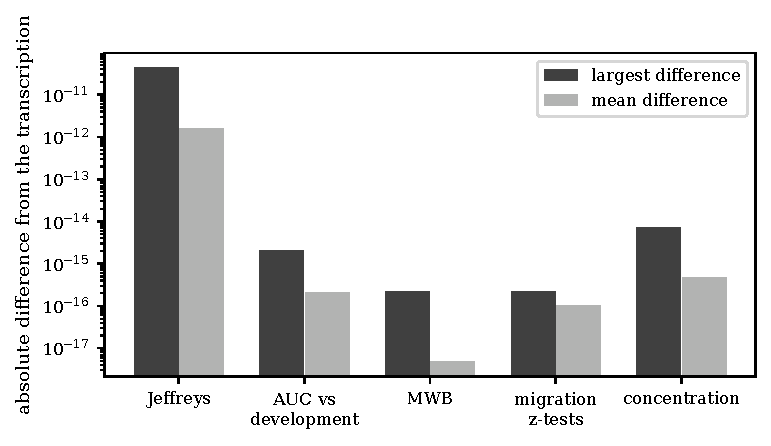
\includegraphics[width=0.8\textwidth]{ecb-agreement}
\caption{Largest and mean absolute difference between each ECB statistic of the engine and an independent transcription of the instructions, over \ecbInputs{} seeded random inputs per statistic, on a logarithmic axis; the Jeffreys bar is the accuracy of the quadrature used by the transcription.}
\label{fig:ecb-agreement}
\end{figure}

\subsection{The Jeffreys test against the nearest generic tests on the credit-card holdout}

On the \cCells{} grade cells of the eight models of the credit-card holdout (every grade with obligors, and the portfolio row of each model) the ECB Jeffreys test flags \flagJeffFive{} cells at the 5\,\% level and the exact one-sided binomial test of SciPy flags \flagBinFive{}; at the 1\,\% level both flag \flagJeffOne{}, so they differ in \disagreeFive{} cell at 5\,\% and in \disagreeOne{} at 1\,\%. The cell that differs is grade \diffGrade{} of the model \texttt{\diffModel{}}, with \diffN{} obligors and \diffD{} defaults, where the binomial $p$-value is \diffPb{} and the Jeffreys value \diffPj{}: the binomial value lies just above the level and the Jeffreys value just below, as Proposition~\ref{prop:sandwich} predicts, and no cell goes the other way. The Jeffreys interval of statsmodels, used as a one-sided limit at 5\,\%, reproduces the engine's decision on \smMatch{} of \cCells{} cells, so the building block exists in a statistics library and what the engine adds is the assembly: the grade-by-grade and portfolio tests with the obligor-weighted portfolio probability and the reporting fields. Figure~\ref{fig:jeffreys-binomial} plots the two $p$-values. The median absolute difference of the two is \medPGap{}, and the largest, \maxPGap{}, occurs in a grade of \worstGapN{} obligors with \worstGapD{} defaults of the model \texttt{\worstGapModel{}} where the two $p$-values are \worstGapPj{} and \worstGapPb{}; the sandwich bounds the difference by the probability of the observed count, which in a grade that small is large. The engine's values equal the committed $p$-values of the case to \committedGap{}. Hypothesis~H2 holds, narrowly: the two tests differ in one cell of \cCells{} at 5\,\% and in none at 1\,\%.

\begin{figure}[htbp]
\centering
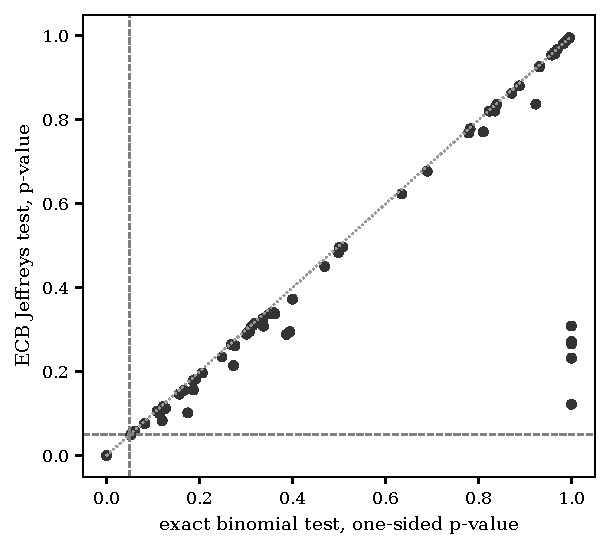
\includegraphics[width=0.55\textwidth]{jeffreys-binomial}
\caption{One-sided $p$-value of the ECB Jeffreys test against that of the exact binomial test for every grade cell of the eight credit-card models of the committed holdout; points lie on or below the diagonal as the sandwich of Proposition~\ref{prop:sandwich} requires, and dashed lines mark the 5\,\% level.}
\label{fig:jeffreys-binomial}
\end{figure}

\subsection{The portfolio engine against anchors, independent routes and its own rung}

The integral of the large-portfolio density equals the engine's distribution function to \lhpMax{} at seven points (Figure~\ref{fig:lhp-anchor}), which is the accuracy of the quadrature. The IRB capital of the credit-card book, at a default probability of \irbPd{} and correlation $0.04$, is \irbK{} by the formula written with SciPy, and the engine's IRB module and its large-portfolio capital differ from it by \irbDiff{}; the identity is exact because all three call the same normal distribution function, so the check holds the wiring and the formula and not the distribution function. The CreditRisk+ recursion returns a probability of no loss of \crpPzero{}, a mean of \crpMean{} loss units and a variance of \crpVar{}, and the variance differs from the closed form of Proposition~\ref{prop:crp} by a relative \crpVarGap{}, with \crpMass{} of probability mass beyond the grid of \crpNmax{} units at $\sigma^2=\crpSigma{}$. The independent recursion of \eqref{eq:crp}, written for the experiment, differs from the stable form by at most \crpIndMax{} in absolute terms over \crpCompared{} probabilities and by a relative \crpIndRel{} over the \crpIndPositive{} that are positive, which is the relative criterion of Hypothesis~H3, and from the engine's Panjer form by \crpIndPanjer{} in absolute terms. The granularity factor is $\delta=\gaDelta{}$ against the printed $4.83$, which agrees to the printed digits, and for identical names the product of the adjustment and the number of names is \gaTimesN{} at 10, 100, 1,000 and 10,000 names with a relative spread of \gaSpread{}.

\begin{figure}[htbp]
\centering
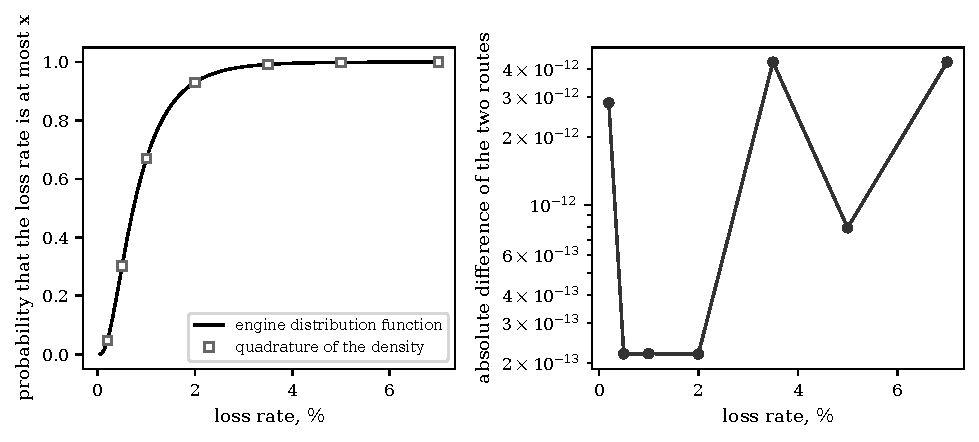
\includegraphics[width=\textwidth]{lhp-anchor}
\caption{Left: the distribution function of the large-portfolio loss rate at the fitted default probability and correlation of the commercial book, with the integral of the engine density computed by adaptive quadrature at seven points. Right: absolute difference of the two routes on a logarithmic axis.}
\label{fig:lhp-anchor}
\end{figure}

The copula sampler is compared with an independent simulator that draws its own normals. Over \mcReps{} runs of \mcScen{} scenarios each, at the correlation \mcRho{} of the one-factor rung, the 99\,\% value at risk is \mcVarNinetyNineEng{} $\pm$ \mcVarNinetyNineEngSd{} for the engine and \mcVarNinetyNineInd{} $\pm$ \mcVarNinetyNineIndSd{} for the independent simulator ($z=\mcVarNinetyNineZ{}$); the 99\,\% expected shortfall is \mcEsNinetyNineEng{} $\pm$ \mcEsNinetyNineEngSd{} and \mcEsNinetyNineInd{} $\pm$ \mcEsNinetyNineIndSd{} ($z=\mcEsNinetyNineZ{}$); the 99.9\,\% value at risk is \mcVarNinetyNineNineEng{} $\pm$ \mcVarNinetyNineNineEngSd{} and \mcVarNinetyNineNineInd{} $\pm$ \mcVarNinetyNineNineIndSd{} ($z=\mcVarNinetyNineNineZ{}$); and the 99.9\,\% expected shortfall is \mcEsNinetyNineNineEng{} $\pm$ \mcEsNinetyNineNineEngSd{} and \mcEsNinetyNineNineInd{} $\pm$ \mcEsNinetyNineNineIndSd{} ($z=\mcEsNinetyNineNineZ{}$). The mean loss is \mcMeanEng{} and \mcMeanInd{} against the exact expected loss of \mcElExact{}. All four $|z|$ values are below one, so the sampler agrees with the independent simulator within the resolution of Proposition~\ref{prop:power} (Figure~\ref{fig:mc-agreement}). The committed rung of \regenN{} scenarios at seed \regenSeed{} and chunk size \regenChunk{} is regenerated by the engine in \regenSeconds{} seconds with a largest relative difference of \regenRel{} over the eight values, the rounding of the committed file; the file holds rounded values, so the comparison cannot show equality of the unrounded sample. The Gaussian importance sampler estimates the probability that the loss exceeds the committed 99.9\,\% value at risk of \isThreshold{} as \isMean{} $\pm$ \isSd{} over \isReps{} seeds, against \isPlainMean{} $\pm$ \isPlainSd{} for plain sampling ($z=\isZ{}$, importance sampler minus plain sampling, the order of the other rows), with a variance ratio of \isRatio{} (Figure~\ref{fig:importance-sampling}); the expected-shortfall contributions of the groups sum to the sample expected shortfall of \eulerEs{} with a relative gap of \eulerGap{}. The Student $t$ importance sampler is not implemented, and the committed rung records that it did not run. Hypotheses~H3 and~H4 hold.

\begin{figure}[htbp]
\centering
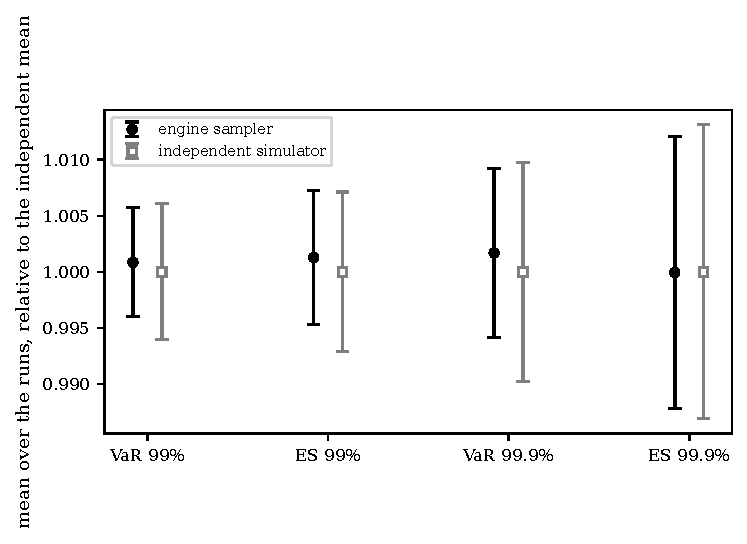
\includegraphics[width=0.8\textwidth]{mc-agreement}
\caption{Mean over \mcReps{} runs of the engine's copula sampler for four risk measures, relative to the mean of an independent simulator written from the model, with one standard deviation over the runs as the bar; the independent simulator sits at one by construction.}
\label{fig:mc-agreement}
\end{figure}

\begin{figure}[htbp]
\centering
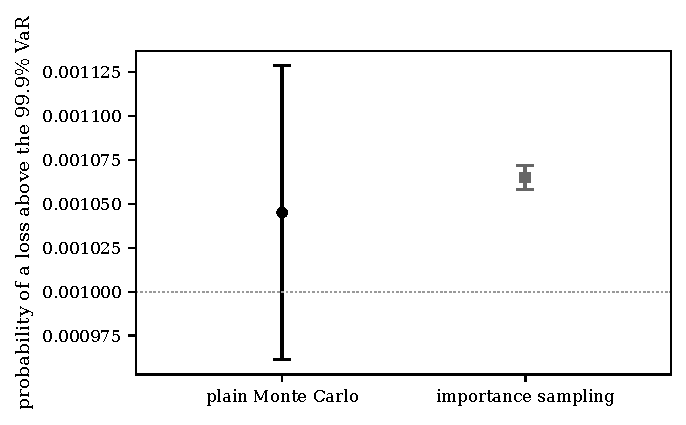
\includegraphics[width=0.6\textwidth]{importance-sampling}
\caption{Estimate of the probability that the portfolio loss exceeds the committed 99.9\,\% value at risk, from plain Monte Carlo and from the Gaussian importance sampler, as the mean over \isReps{} seeds of \isScen{} scenarios with one standard deviation as the bar; the dotted line is the nominal 0.1\,\%.}
\label{fig:importance-sampling}
\end{figure}

\subsection{The correlation estimator against a known truth}

Table~\ref{tab:grid} and Figure~\ref{fig:coverage-grid} give the coverage of the nominal 95\,\% interval in the committed simulator. The maximum-likelihood estimator has a mean coverage of \gridMlMeanCov{} over the \gridMlCells{} cells and its coverage is outside the 99\,\% band of $\pm\gridBandHalf{}$ in \gridMlFail{} of them: the lowest is \gridMlWorstCov{} at a true correlation of \gridMlWorstRho{} with series of \gridMlWorstYears{} years ($z=\gridMlWorstZ{}$). The coverage is below $0.95$ in \gridMlBelow{} of the \gridMlCells{} cells and the bias is negative in \gridMlNegBias{} of them, from \gridMlBiasMin{} to \gridMlBiasMax{}, so the estimator undercovers throughout the grid and not in one cell. Pooled over the \gridMlPooledReps{} replications of all cells the coverage lies $\gridMlPooledZ{}$ binomial standard errors from $0.95$, a figure that holds only if the cells are independent, which was not checked: one seed drives the 22-year grid. At a correlation of 0.24 and 22 years the coverage is \gridMlCovTwentyFour{} and the bias \gridMlBiasTwentyFour{}. The moments estimator has a mean coverage of \gridMomMeanCov{}, is outside the band in \gridMomFail{} of \gridMomCells{} cells, and its lowest coverage is \gridMomWorstCov{} at a correlation of \gridMomWorstRho{} with series of \gridMomWorstYears{} years; at 0.24 and 22 years its bias is \gridMomBiasTwentyFour{} and its coverage \gridMomCovTwentyFour{}. The re-run of three 22-year cells with \cellReps{} fresh replications gives coverages of \cellLowCov{} $\pm$ \cellLowCovSe{}, \cellMidCov{} $\pm$ \cellMidCovSe{} and \cellHighCov{} $\pm$ \cellHighCovSe{} at correlations of 0.02, 0.12 and 0.24, and biases of \cellLowBias{} $\pm$ \cellLowBiasSe{}, \cellMidBias{} $\pm$ \cellMidBiasSe{} and \cellHighBias{} $\pm$ \cellHighBiasSe{}. Hypothesis~H5 is refuted: \gridMlFail{} of \gridMlCells{} cells lie outside the band where \gridChance{} are expected by chance, and the mean coverage and the sign of the bias show an undercoverage that the single cell understates. The cell outside the band is the one at the lowest correlation with 22 years, and the re-run at that correlation is below $0.95$ as well.

\begin{table}[htbp]
\centering
\small
\caption{Coverage of the nominal 95\% interval at three of the twelve known correlations of the committed simulator, for 22 and 40 years, with 400 replications per cell; z is the distance of the coverage from 0.95 in binomial standard errors.}
\label{tab:grid}
\begin{tabular}{rrrrrr}
\toprule
Years & True correlation & ML coverage & z & Moments coverage & z \\
\midrule
22 & 0.020 & 0.912 & -3.441 & 0.823 & -11.700 \\
22 & 0.120 & 0.948 & -0.229 & 0.815 & -12.388 \\
22 & 0.240 & 0.940 & -0.918 & 0.655 & -27.071 \\
40 & 0.020 & 0.943 & -0.688 & 0.858 & -8.488 \\
40 & 0.120 & 0.940 & -0.918 & 0.870 & -7.341 \\
40 & 0.240 & 0.950 & 0.000 & 0.820 & -11.930 \\
\bottomrule
\end{tabular}
\end{table}


\begin{figure}[htbp]
\centering
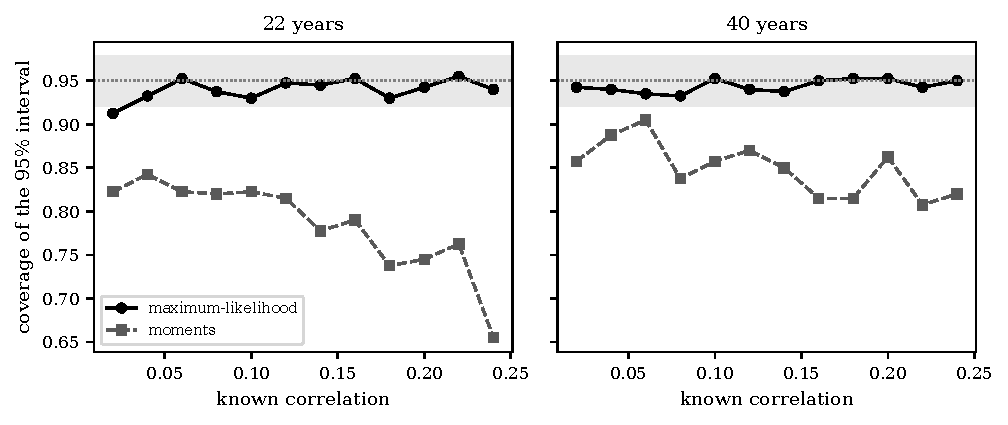
\includegraphics[width=\textwidth]{coverage-grid}
\caption{Coverage of the nominal 95\,\% interval of the asset correlation by the maximum-likelihood and the moments estimators against the known correlation of the committed simulator, for series of 22 and 40 years with \gridReps{} replications per cell; the shaded band is the 99\,\% binomial band around 0.95.}
\label{fig:coverage-grid}
\end{figure}

\subsection{The IRRBB engine against the standard and against QuantLib}

At a mid-point of 3.5 years the engine returns $\alpha_{\mathrm{s}}=\irrAlpha{}$, a short-up shock of \irrShort{} basis points, a steepener of \irrSteep{} and a flattener of \irrFlat{}, against the printed 0.417, 41.7, 25.4 and $-1.6$: the deviations are \irrAlphaDev{}, \irrShortDev{}, \irrSteepDev{} and \irrFlatDev{}, each inside the half-unit of the last printed digit (0.0005 for the factor and 0.05 basis points for the shocks). The transcription of the shocks written for the experiment equals the engine's values to the last digit shown. Over the \irrVariants{} committed variants, two currency legs and six shocks, that is \irrLegs{} leg and shock pairs, the shock shape stored in the artifact equals the engine's to \irrShapeEng{} and equals the transcription to \irrShapeInd{}; the engine's present value equals the stored one with a relative difference of \irrEngMax{}, as the artifact was written by the same function, and the QuantLib present value differs from the stored one by a relative \irrQlMax{} at most (Figure~\ref{fig:eve-reconciliation}). The pair rule that combines the peso and UF legs returns the stored value with a difference of \irrPair{}. Hypothesis~H6 holds, with the limit that QuantLib's present value is the same exponential discounting and so holds the time convention and the wiring of the engine and not the choice of continuous compounding.

\begin{figure}[htbp]
\centering
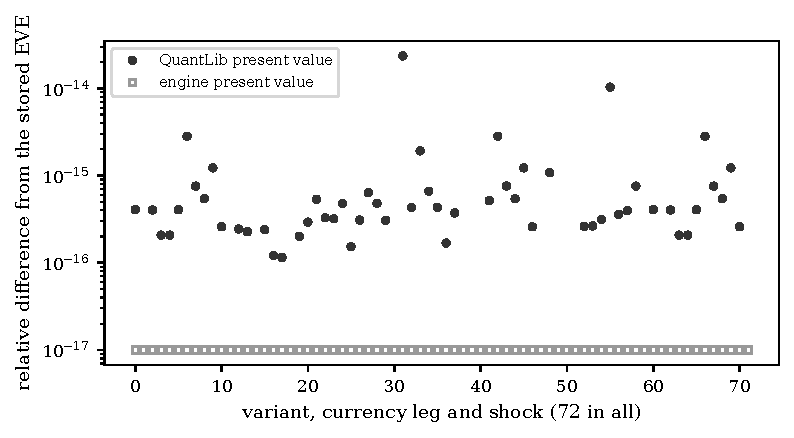
\includegraphics[width=0.85\textwidth]{eve-reconciliation}
\caption{Relative difference between the stored economic value of equity of each of the 72 leg and shock pairs of the six committed interest rate risk variants and the engine's present value and the QuantLib present value of the same cash flows, on a logarithmic axis; zero differences are drawn at the axis floor.}
\label{fig:eve-reconciliation}
\end{figure}

\subsection{The open toolkits}

The survey queried \pypiQueried{} package names on \pypiDate{}, of which \pypiFound{} exist on PyPI; the \pypiMissing{} that do not are \pypiMissingNames{}. Table~\ref{tab:toolkits} sets the vocabulary of the catalogue against the \distScanned{} installed distributions, whose \filesScanned{} Python files were scanned, and against the summary and long description of the \pypiFound{} packages. In the installed sources the word Jeffreys appears in the statistics library for the proportion and rate intervals, Herfindahl in the binning library for a concentration index of the bins, Vasicek in the SciPy entropy estimator of that name and not in the credit model, and the weighted-matrix words in a graph test. In the package texts, the only package that names the Jeffreys test, CreditRisk+, the granularity adjustment, the Vasicek model, the ECB or the interest rate risk in the banking book is the engine itself. Hypothesis~H7 is not refuted by this survey; its limits are those of a search of metadata and of an installed environment, and Section~\ref{sec:limitations} states them.

\begin{table}[htbp]
\centering
\small
\caption{Where the catalogue's vocabulary appears in the Python sources of 106 installed distributions and in the PyPI summary and description of 34 toolkits read on 2026-11-06; a match is a word, not an implementation of the specified test.}
\label{tab:toolkits}
\begin{tabular}{lrlrl}
\toprule
Vocabulary & Installed packages with a match & Which & PyPI texts with a match & Which \\
\midrule
jeffreys & 1 & statsmodels & 1 & riskvalidation \\
herfindahl & 1 & optbinning & 0 & -- \\
matrix weighted bandwidth & 1 & networkx & 0 & -- \\
creditrisk+ & 0 & -- & 1 & riskvalidation \\
granularity adjustment & 0 & -- & 1 & riskvalidation \\
vasicek & 1 & scipy & 1 & riskvalidation \\
irrbb & 0 & -- & 1 & riskvalidation \\
economic value of equity & 0 & -- & 0 & -- \\
somers d & 2 & scipy, statsmodels & 0 & -- \\
migration matrix test & 0 & -- & 0 & -- \\
\bottomrule
\end{tabular}
\end{table}

